\RequirePackage{plautopatch}

\documentclass[a4paper, 11pt]{ltjsarticle}


% マージン設定
\usepackage[top=20mm, bottom=20mm, left=30mm, right=10mm]{geometry}

% LuaLaTeX用日本語対応パッケージ
\usepackage{luatexja}
\usepackage{luatexja-fontspec}

% 必要なパッケージ
\usepackage{fontspec}
\usepackage{titlesec}
\usepackage{graphicx}
\usepackage{amsmath}
\usepackage{amssymb}
\usepackage[colorlinks=true, linkcolor=black, citecolor=black]{hyperref}
\usepackage{tocloft}
\usepackage{indentfirst}
\usepackage{tikz} % カスタム点線用
\usepackage{here}
\usepackage{subcaption}
\usepackage{bookmark}
\usepackage{booktabs}
\usepackage{multicol}
\usepackage{multirow}
\usepackage{flushend}
\usepackage{threeparttable}
\usepackage{enumitem}
\usepackage{pifont}  % 丸囲み数字を使うためのパッケージ
\usepackage{url}
\usepackage{svg}
\usepackage{makecell}

% 図:1のコロンを消す
\captionsetup{labelsep=space}

% 参考文献を上付きにする
\usepackage[super]{cite}
\renewcommand\citeform[1]{[#1]}

\setlength{\baselineskip}{14pt}
\setlength{\parindent}{1\zw}

\titleformat{\section}{\large\bfseries}{\thesection.}{1\zw}{}
\titleformat{\subsection}{\large\bfseries}{\thesubsection.}{1\zw}{}
\titleformat{\subsubsection}{\large\bfseries}{\thesubsubsection.}{1\zw}{}

\setcounter{tocdepth}{3}
\makeatletter
\renewcommand{\numberline}[1]{#1.~}
\renewcommand{\cftsecleader}{\cftdotfill{\cftdotsep}}
\renewcommand{\cftsubsecleader}{\cftdotfill{\cftdotsep}}
\renewcommand{\cftsubsubsecleader}{\cftdotfill{\cftdotsep}}
\makeatother

\DeclareCaptionFont{designatedFont}{\fontsize{11pt}{14pt}\selectfont}
\captionsetup{font=designatedFont}

%---ここから中身---------------------------------------------------------------------------------------
\begin{document}
\fontsize{11pt}{14pt}\selectfont

%---表紙---------------------------------------------------------------------------------------
\thispagestyle{empty}
\begin{center}
\pagenumbering{gobble}  %ページ番号をカウントしない

\vspace*{40mm}
{\huge\noindent 災害時を想定したアドホックネットワーク}\\
\medskip
{\huge\noindent 構築手法の検討}\\
\vspace{\baselineskip}
{\huge\noindent\textbf{Study of Construction Methods for Ad-Hoc Network under Disaster}}\\
\vspace{120mm}

{\huge\noindent
2025年3月4日\\
東京都立産業技術高等専門学校\\
ものづくり工学科 情報通信工学コース \\
末廣 隼人\\
指導教員 髙﨑 和之    \\
}
\vspace{40mm}

\end{center}

%---目次------------------------------------------------------------------------------------------
\clearpage  %新しいページの追加
\thispagestyle{empty}
\tableofcontents  %目次の自動生成 目次をクリックするとその章,節に飛ぶことができる

%---はじめに---------------------------------------------------------------------------------------
\clearpage
\pagenumbering{arabic}
\section{はじめに}

% ・日本では地震をはじめ多くの自然災害が発生しており,災害時には通信ネットワークが使えなくなる可能性がある.
% そこで,アドホックネットワークを活用し地域限定ながら被災状況の把握や情報伝達を可能とする研究が行われている.\\
% ・本研究では,人口密度に応じた経路構築方法を考案し,その効果をシミュレーションを用いて検証した.\\
% ・近年,Bluetoothの開発が活発に行われており,従来のBluetooth Basic Rate/Enhanced Data Rate(BR/EDR)と比べて
% 大幅な省電力化が行われたBluetooth Low Energy(BLE)が発表された.そして,\\
% ・地震などの大きな災害が発生した際,従来の基地局を用いたネットワークへのアクセスの集中等により使用できなくなった場合,
% 新たなコミュニケーション環境の実現手段として,アドホックネットワークの研究が行われている.
・実際の環境でアドホックネットワークを構築することが難しいため,シミュレーションを通して有効的な
経路構築方法が何か,また,安定した通信を行うにはどのような条件が必要なのかを確認した.
・地震等の大規模災害発生時に


%---理論---------------------------------------------------------------------------------------
\clearpage
\section{理論}
\subsection{アドホックネットワークについて} \label{about_ad-hoc}
アドホックネットワークとは,中央の管理者やルータ,アクセスポイントなどの既存のインフラストラクチャを介さずに,
端末(以下では,ノードと呼ぶ)同士が直接通信を行う一時的なネットワークのことである.
電波が届かず直接情報を交換できないノード同士の場合,基地局を経由せずに途中のノードが中継するマルチホップ通信により情報交換が可能になる.

これらを踏まえると,ノードさえあればどのようなエリアでも即席にネットワークを形成することができるためとても便利だが,
ノード移動に伴うネットワークトポロジや伝送品質の急激な変化,利用可能な無線周波数帯域の限界,バッテリ依存によるノードの消費電力などの制約といった
厳しい条件がある.そのため,ルーティングやチャネルアクセスの制御,周波数帯域の有効活用,ノードの電力消費の節約等の多くの課題がある\cite{間瀬憲一2001アドホックネットワーク}.

アドホックネットワークに関する研究の歴史は長く,アドホックネットワークの第一世代であるPRNET(Packet Radio Network)
は,1972年に米国の国防高等研究計画局によって開発され,軍事利用を目的とした研究のために開始された.
次に,第二世代であるNTDR(Near-term Digital Radio)も,米国により軍事目的で研究が行われ,1980年代頃に実用化された.
そして,第三世代であるMANET(Mobile Ad hoc NETwork)を含む現在のアドホックネットワーク技術は,IEEE802.11やBluetoothなどの
近距離無線通信技術を活用し,民間でも使用できるアドホックネットワークが2000年頃から誕生した.
加えて,同時期から災害時用ネットワークとしての活用に期待が高まっていた.

\subsection{ルーティングプロトコル}
アドホックネットワークには,ネットワークトポロジの急激な変化や消費電力の増加など,経路の構築前,構築後で
の課題が多く残っている.
そのため,アドホックネットワークを効率的に構築,運用するために,ルーティングプロトコルが用いられている.
図\ref{routing_classification}にルーティングプロトコルの分類とプロトコルの代表例を示す.

ルーティングプロトコルは,大きくリアクティブ型,プロアクティブ型,ハイブリッド型の3つに分類される.
それぞれ,経路探索のタイミングや管理方法が異なり,スループットやオーバーヘッドなどに影響を与える.
次項にそれぞれの特徴と簡単な概略図を用いて紹介を行う.
\begin{figure}[H]
  \centering
  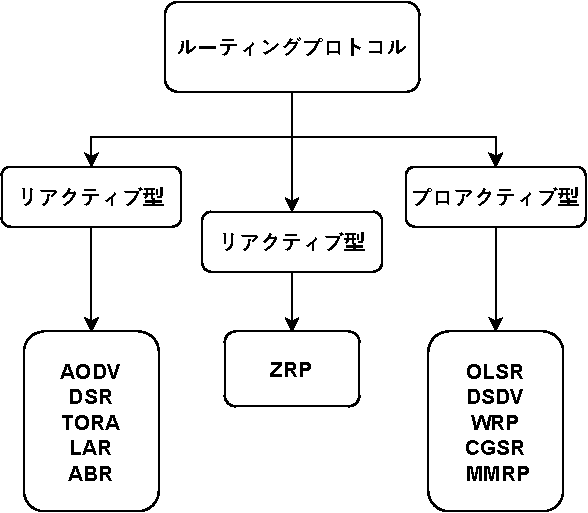
\includegraphics[width=85mm]{classification_of_routing.pdf}
  \caption{ルーティングプロトコルの分類}
  \label{routing_classification}
\end{figure}

\clearpage
\subsubsection{リアクティブ型}
あるノードが通信要求を行なった時にルーティングプロトコルに基づいて電波をフラッディングし,
近隣のノードとその場で情報のやり取り行い経路生成を行う.
通信要求がなされた時に作成されるため,実際に通信が開始されるまでにラグが発生する.

このようにする理由として,アドホックネットーワークを構築するノードのデバイスがバッテリなどで駆動することが多いため,
むやみやたらに電波をフラッディングしてしまうと,電池の消費速度が速くなってしまうからである.
加えて,ノードの移動により,ネットワークが動的に変化変化しまうため,
数分前に構築された経路表の有効性が失われる場合が多い.したがって,
通信直前に経路表を生成することで電波のフラッディング回数を減らし,駆動時間の長時間化が行われる.
それゆえに,通信開始が遅くても良い環境で用いられている.

リアクティブ型での動作イメージを図\ref{reactive}に示した.
ノードA \textasciitilde Eが図のようにある時,ノードAとEが通信を行う場合を考える.
次に,リアクティブ型での経路構築の手順を示す.

\begin{enumerate}[label=\ding{\numexpr171+\arabic*}]
  \item \label{1} ノードAが自身のIDと宛先ノードの情報を載せてフラッディングを行う.
  \item \label{2} \ref{1}の情報を受信したノードは,送信元を記録してから,宛先を確認する.
  今回の場合,宛先が違うため①と同様の情報を載せてフラッディングを行う.\\
  宛先のノードに辿り着くまで行う.
  \item \label{3} \ref{2}の情報を受信したノードEは,今回の宛先であるため,これまでの経路を逆順に辿って行き,
  発信元のノードAに経路が生成されたことを伝達し,経路表をもとに通信を行う.
\end{enumerate}

\begin{figure}[H]
  \centering
  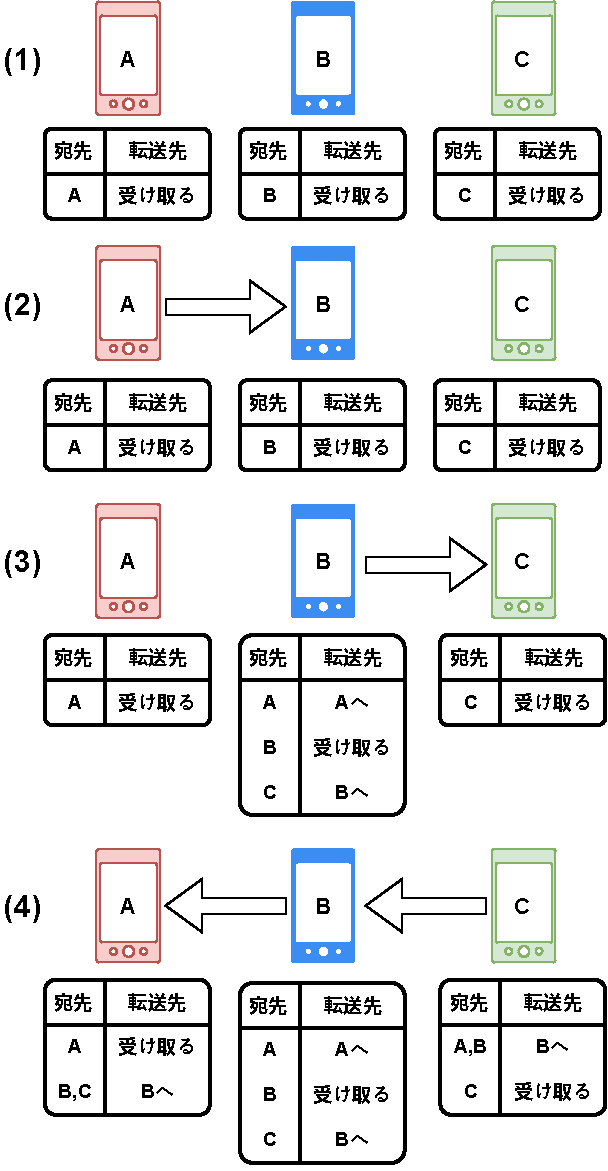
\includegraphics[width=130mm]{reactive_model.pdf}
  \caption{リアクティブ型の動作イメージ図}
  \label{reactive}
\end{figure}

ノードC, Dはノードが存在する限りフラッディングを行なってしまうため,現在の情報にフラッディングをする回数も同時に
送信し,回数が0になったら,これ以上の探索は実施しないという対策が必要となる.

代表的なプロトコルとしてAODV,DSR,TORA,LAR,ABRなどがある.次にそれぞれの特徴について概説する.

\begin{itemize}
  \item AODV(Ad hoc On-Demand Distance Vector)\cite{AODV} \\
  \item DSR(Dynamic Source Routing)\cite{DSR} \\
  \item TORA(Temporally-Ordered Routing Algorithm)\cite{TORA} \\
  \item LAR(Location-Aided Routing)\cite{LAR} \\
  \item ABR(Associativity-Based Routing)\cite{ABR} \\
\end{itemize}

\clearpage
\subsubsection{プロアクティブ型}
リアクティブ型では通信要求が発生してから経路表が作成されるのに対し,プロアクティブ型では近隣のノードと周期的に情報のやり取りを行い,
通信要求が発生したらすぐに通信を開始することができる.しかし,リアクティブ型と比べ頻繁に情報のやり取りを行うため,電池の消費が早い.
常に新鮮な経路表を保持しているためノードの入れ替わりが激しい環境では有効的である.

以下にリアクティブ型での動作イメージを図\ref{proactive}に示した.各ノードは常に近隣のノードと情報をやり取りしているため,
通信の開始が早く,また,近隣のノードが接続が不可能になったとしても,すぐに新たな経路を生成することが可能であり安定した通信を行うことができる.
\begin{figure}[H]
  \centering
  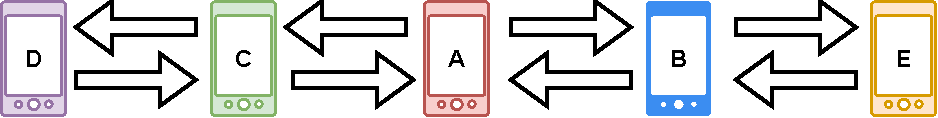
\includegraphics[width=130mm]{proactive_model.pdf}
  \caption{プロアクティブ型の動作イメージ図}
  \label{proactive}
\end{figure}

代表的なプロトコルとしてOLSR,DSDV,WRP,CGSR,MMRPなどがある.

\begin{itemize}
  \item OLSR(Optimized Link State Routing)\cite{OLSR}\\
  \item DSDV(Destination-Sequenced Distance-Vector)\cite{DSDV}\\
  \item WRP(Wireless Routing Protocol)\cite{WRP}\\
  \item CGSR(Cluster-head Gateway Switch Routing)\cite{CGSR}\\
  \item MMRP(Mobile Mesh Routing Protocol )\cite{MMRP}\\
\end{itemize}

\subsubsection{ハイブリッド型}
リアクティブ型とプロアクティブ型の長所を組み合わせたプロトコルである.
代表的なプロトコルとしてZRP(Zone Routing Protocol)\cite{1574231874891177344}がある.

ZRPでは,ネットワークをゾーンと呼ばれる単位で分割し,ゾーン内にあるノードに対してはプロアクティブ型のルーティングプロトコルで近隣の情報同士でやり取りを行い,
ゾーン外にあるノードに対してはリアクティブ型のルーティングプロトコルで通信要求が発生した場合のみ動作しそのノードまでの経路を生成する.

メリットとして,ゾーン内では短距離通信の遅延が最小化され,ゾーン外では不要な情報のやり取りを減らすことが可能となる.
また,ネットワークが大規模になったとしても全ての経路情報を保持しなくて良いため効率的に運用することが可能である.
しかし,デメリットとして,ゾーン半径の設定が困難であることである.
ゾーン半径が小さい場合,遠距離通信が頻繁に発生してしまい,また,
ゾーン半径が大きい場合,ゾーン内に存在するノードが多数になり計算コストとメモリ消費が増大する可能性がある.

\begin{figure}[H]
  \centering
  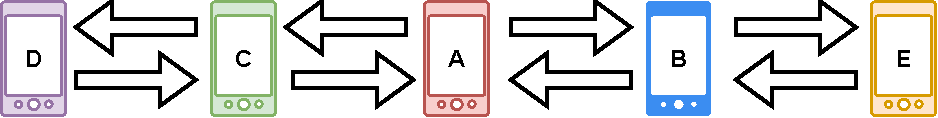
\includegraphics[width=80mm]{proactive_model.pdf}
  \caption{ハイブリッド型の動作イメージ図(仮)}
  \label{hybrid}
\end{figure}

\clearpage
\subsection{アドホックネットワークの技術的課題}
\ref{about_ad-hoc}節で述べた課題のほかに,隠れ端末問題とさらし端末問題があり,
これらがアドホックネットワークが一般的に普及されていない原因の一つとも言える\cite{松井_進2012KJ00008330022}.
次項にそれぞれの問題について説明する.
\subsubsection{隠れ端末問題}
図\ref{hidden_problem}に隠れ端末問題を表した図を示す.図\ref{hidden_problem}では,
スマートフォンがノード,その周りにある円がノードからの通信距離を表している.
ノードBの円は見やすさの都合上省略している.

隠れ端末問題とは,ノードAとCがノードBに接続を行うとき,ノードA,Cは互いに通信可能距離外にあるため
互いの存在が隠れてしまい,ノードBが誰とも通信をしてないと判断してしまう.
そして,ノードA,Cが同時にデータをノードBに送信した場合,電波干渉やデータの衝突する問題が発生がある.

この問題により通信制御のスループット(処理能力)の低下が発生し,通信に遅延が生じる.
\begin{figure}[H]
  \centering
  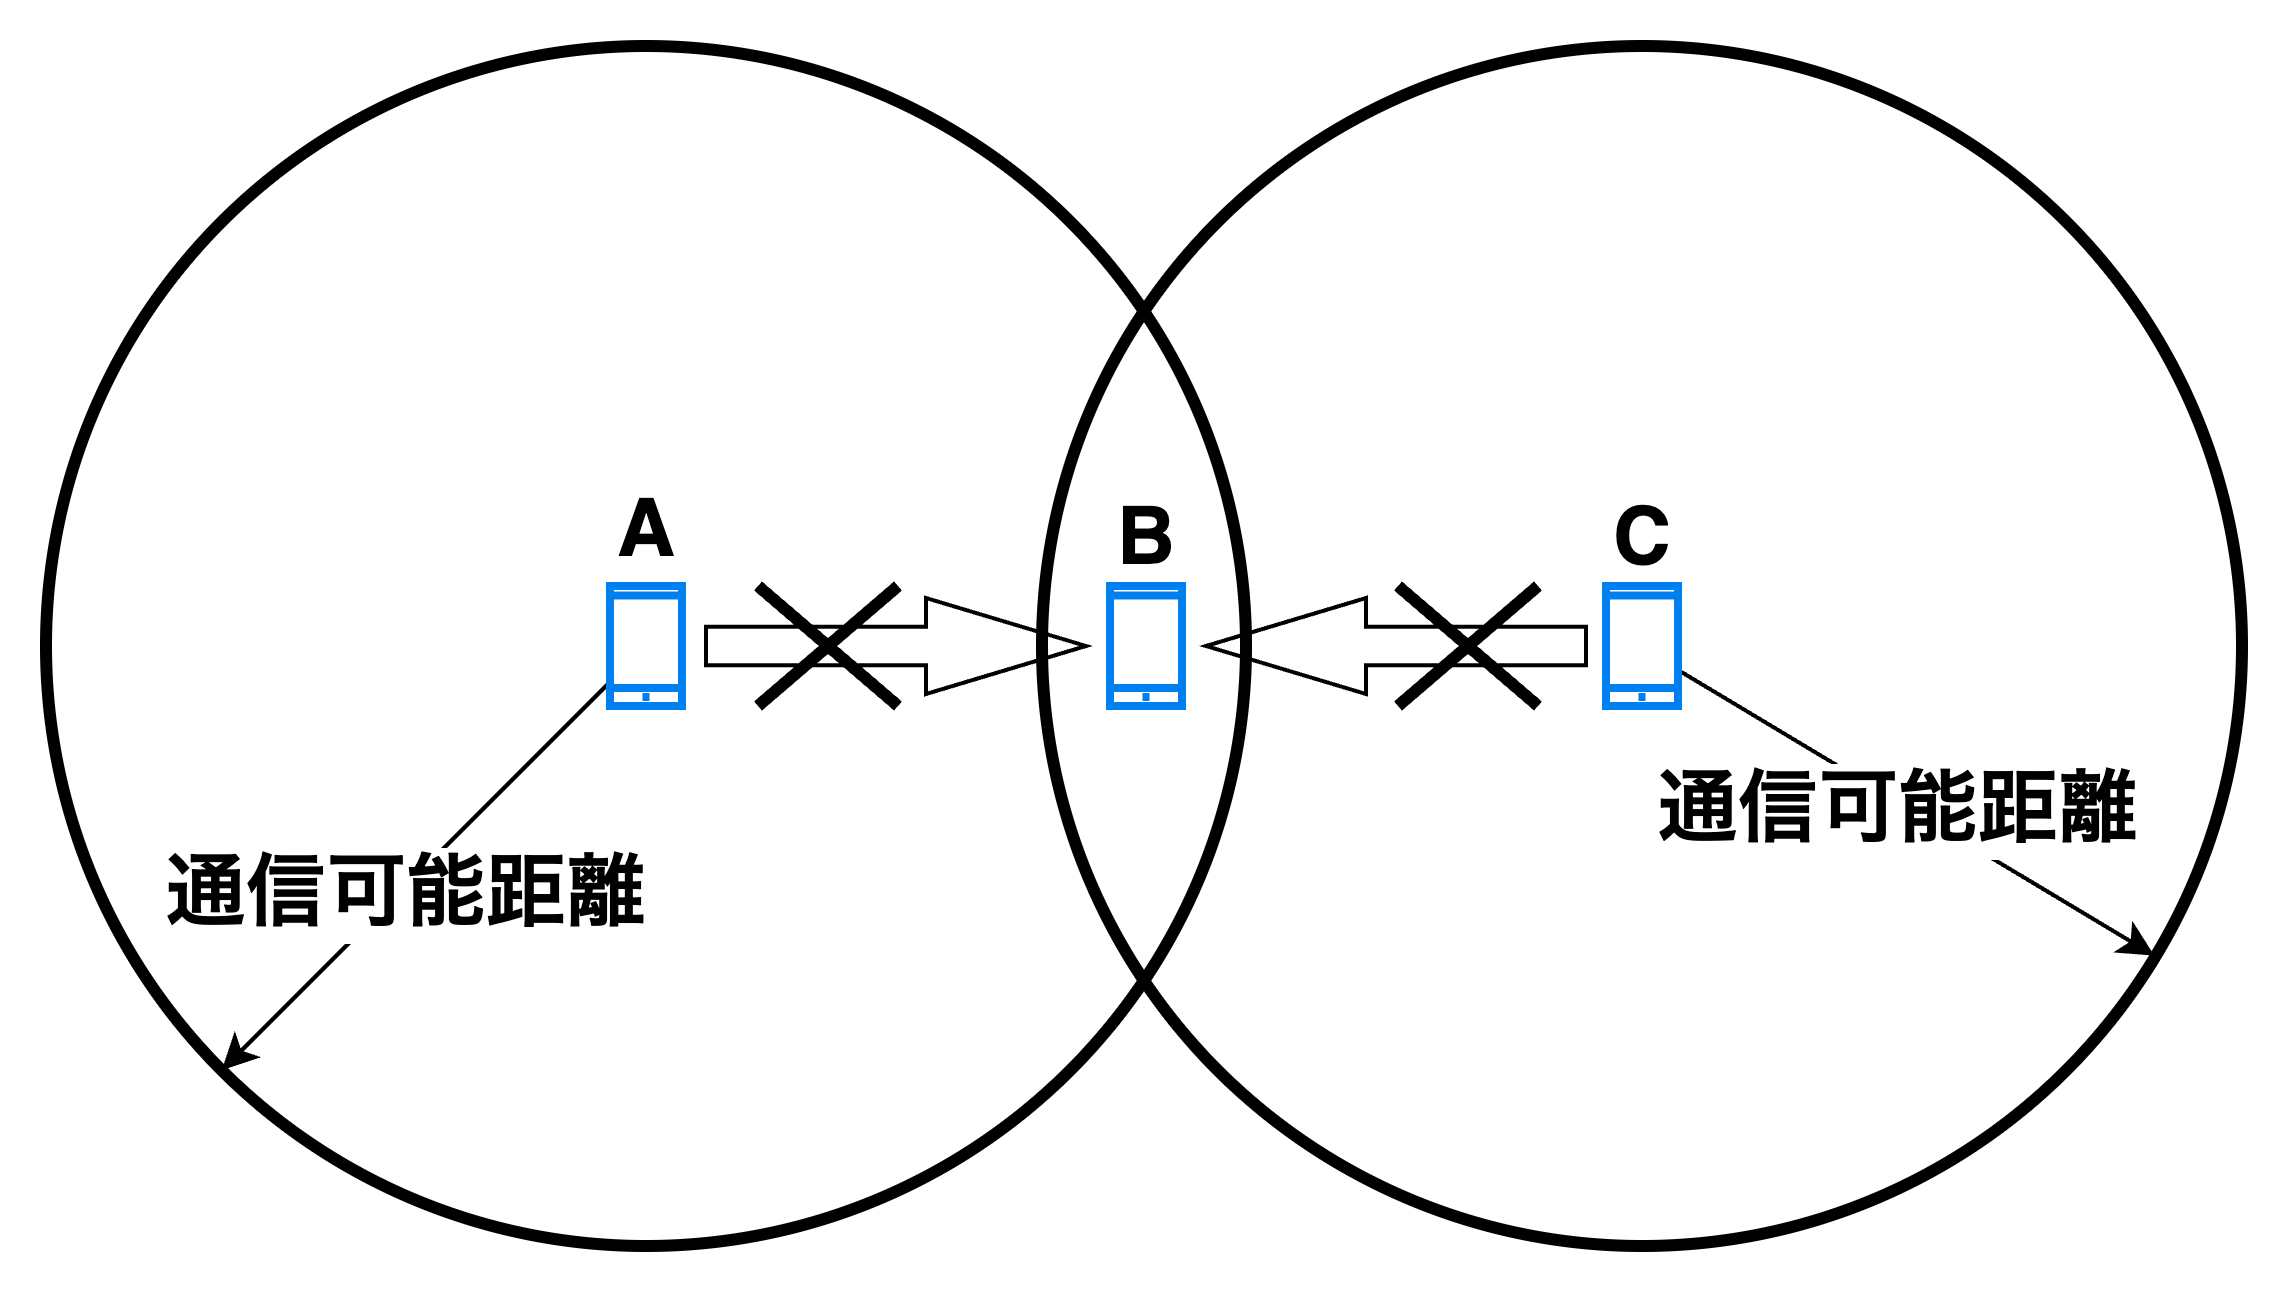
\includegraphics[width=100mm]{hidden_terminal_problem.png}
  \caption{隠れ端末問題}
  \label{hidden_problem}
\end{figure}

\subsubsection{さらし端末問題}
図\ref{exposed_problem}にさらし端末問題の図を示す.
図\ref{exposed_problem}で表されているスマートフォンや円は隠れ端末の場合と同様の意味である.

さらし端末問題とは,ノードA,Dが通信を行っているとき,通信可能距離内にいるノードBは
データを送信して衝突しないようにするために通信抑制が頻繁に行われる問題がある.これにより
伝送速度や通信品質の低下が発生してしまう.
\begin{figure}[H]
  \centering
  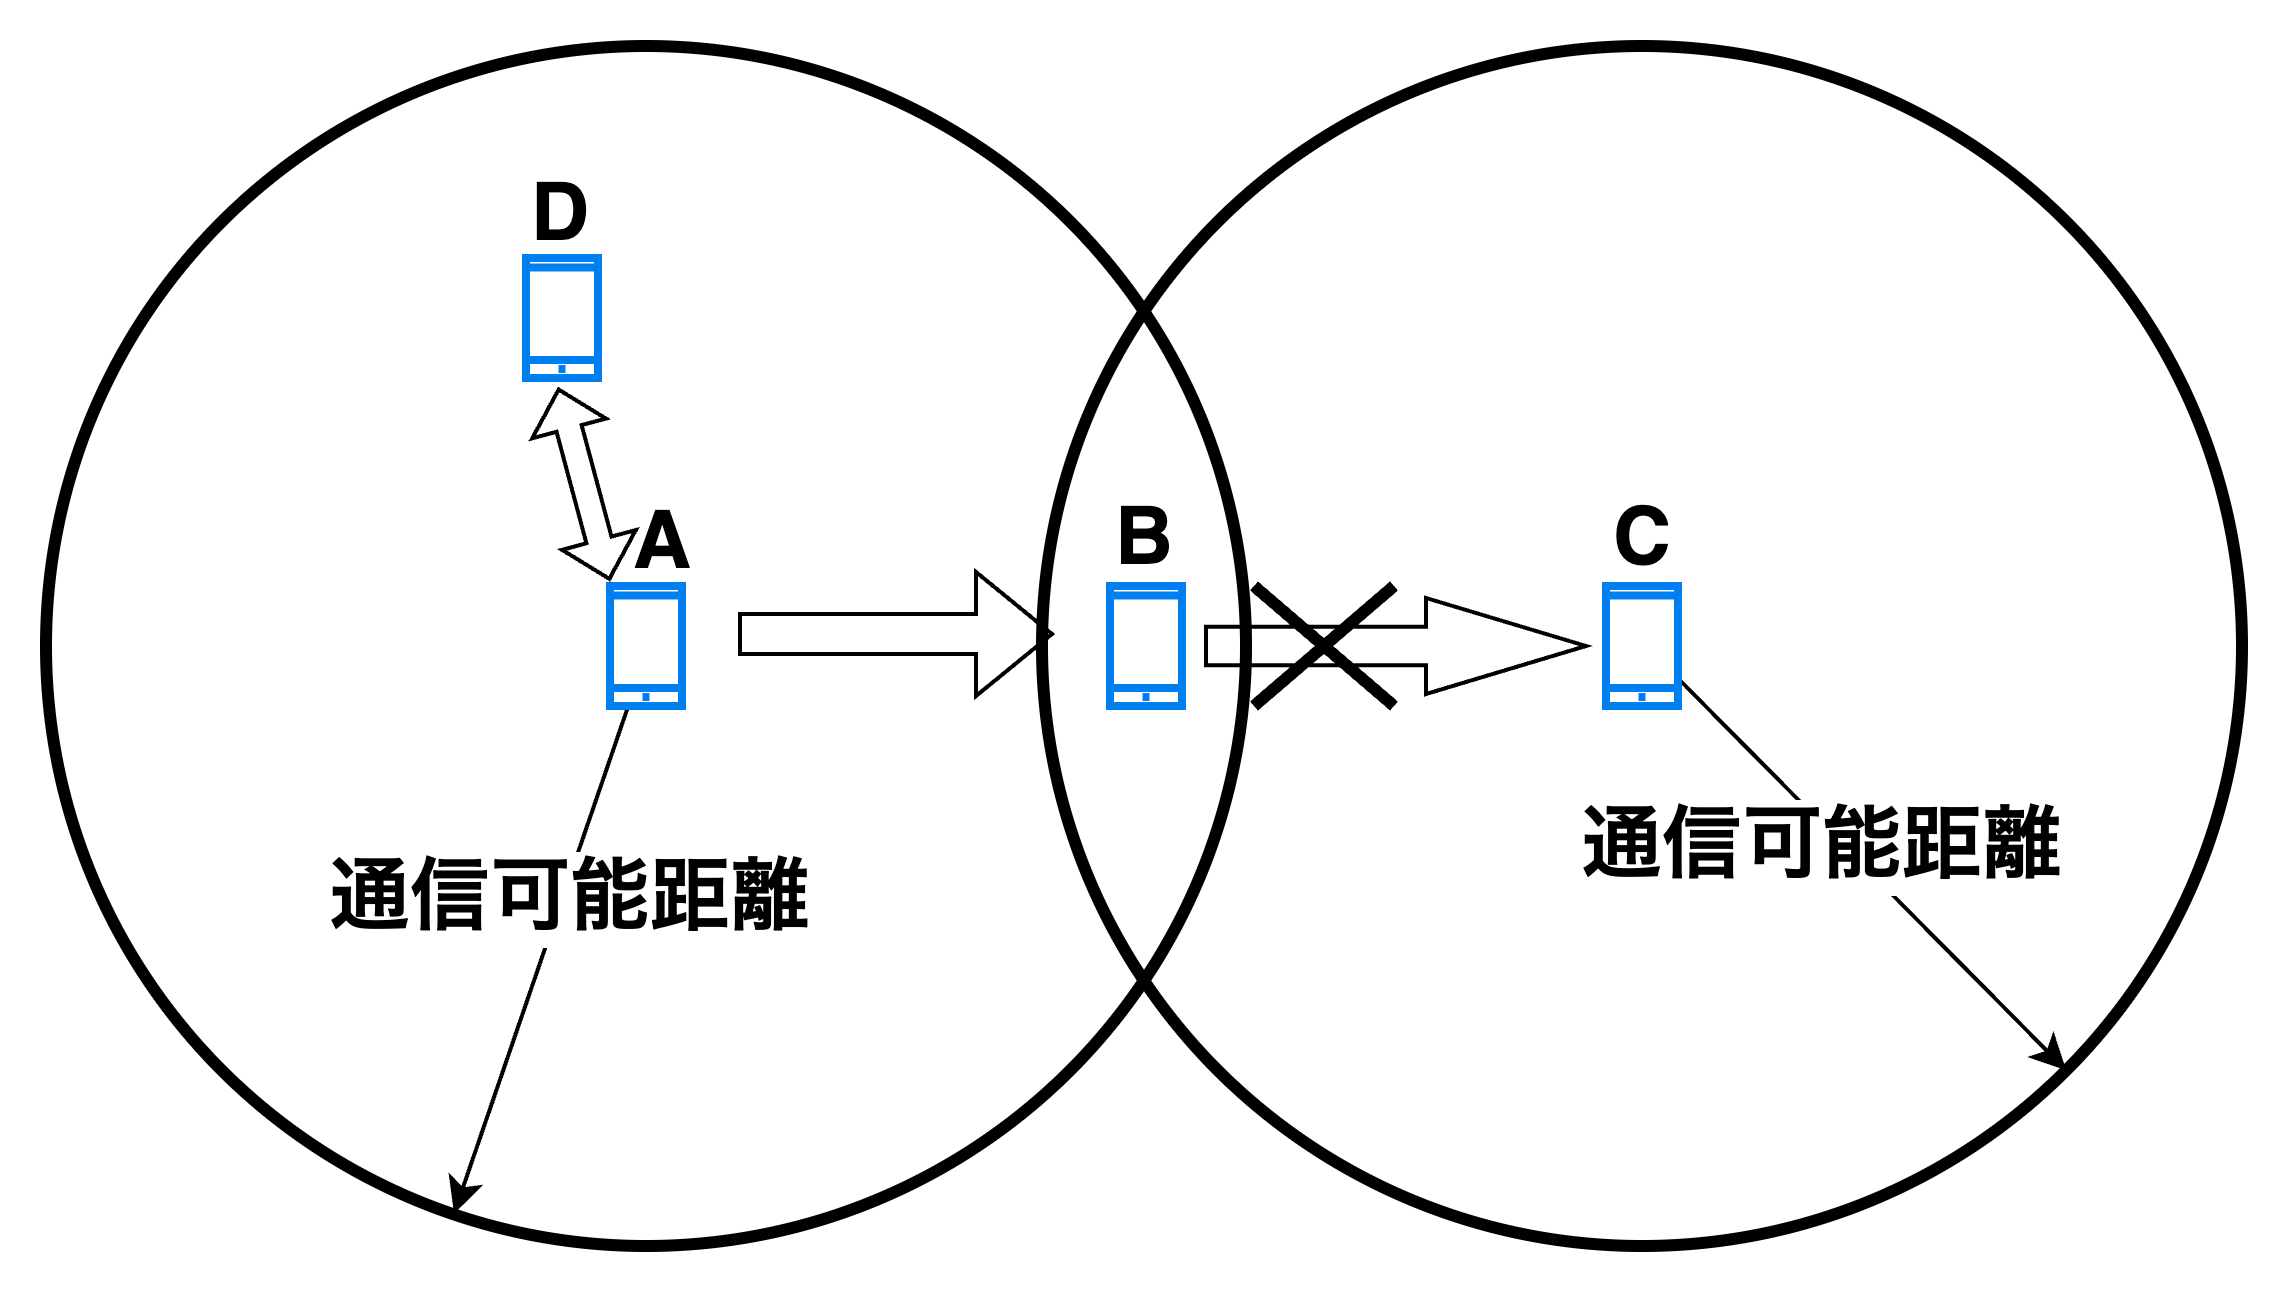
\includegraphics[width=100mm]{exposed_terminal_problem.png}
  \caption{さらし端末問題}
  \label{exposed_problem}
\end{figure}

\clearpage
\subsection{Bluetooth}
Bluetoothとは,デジダル機器用の近距離通信規格の一つであり,数メートルから数十メートル程度での距離間で電波を用いて簡易的な情報のやり取りを行う.
また,免許を必要としない2.4GHzの周波数帯を使用するのでPCのマウスやキーボード,ワイヤレスイヤホン,スマートウォッチなど生活の身近に使用されている.
IEEEの規格名はIEEE802.1.15である.

1994年にスウェーデンのEricsson社が近距離無線通信規格の開発をはじめ,
1998年にPromoter5社(Ericsson,Intel,IBM,Nokia,東芝)によりBluetooth SIG(Special Interest Group)
が設立され,Bluetothの規格策定が行われている.そして,現在まで公開されている仕様として,
Bluetooth ClassicとBluetooth Low Energy(LE)の2種類に分けることができ,
表\ref{Bluetooth_characteristics}にそれぞれの特徴を示した.

\begin{table}[h]
  \centering
  \caption{Bluetooth ClassicとBLEの特徴\cite{Bluetooth_official}}
  \begin{tabular}{c|c|c}
    \specialrule{1.5pt}{0pt}{0pt} % 上端の太線(1.5pt)
       & Bluetooth Classic & BLE \\
      \hline
      周波数帯 & \multicolumn{2}{c}{2.4GHz (2.402 \textasciitilde 2.480GHz)} \\
      \hline
      チャネル利用 & \multicolumn{2}{c}{周波数ホッピングスペクトラム拡散 (FHSS)} \\
      \hline
      チャネル数 & 1MHz間隔で79チャネル & \makecell{2MHz間隔で40チャネル\\(3つはアドバタイジング用チャネル)} \\
      \hline
      転送速度 & 3, 2, 1 Mbps &  2, 1 Mbps,500, 125 kbps \\
      \hline
      同時接続台数 & 最大7台 & 仕様上無限 \\
      \hline
      消費電力 & 1W & 0.01W \textasciitilde 0.5W \\
      \hline
      通信トポロジ & スター型 & スター型,メッシュ型 \\
      \hline
      主な用途 & マウス,イヤホンなど & IoTセンサ,スマートウォッチなど \\
      \specialrule{1.5pt}{0pt}{0pt} % 上端の太線(1.5pt)
  \end{tabular}
  \label{Bluetooth_characteristics}
\end{table}

\subsubsection{Bluetooth Classic}
Bluetooth Classicは,1997年に一般公開されたBluetooth 1.0から3.0までのバージョンを指している.

デバイスには,接続を要求する親機(Master)と接続を受信する子機(Slave)の2種類があり,Masterはいわゆるスマートフォンで,
Slaveはワイヤレスイヤホン等のガジェットに相当するものである.この時,Masterは同時に最大7台のSlaveと接続が可能.
また,Bluetoothで位置検出を行う研究が行われている\cite{勝野_恭治2002}.

通信距離はClass1\textasciitilde3のように電波強度で分類され表\ref{Classic_connecting_distance}のようになっている.

\begin{table}[h]
  \centering
  \caption{Bluetooth Classicの場合\cite{東芝情報システム株式会社}}
  \begin{tabular}{c|l}
    \specialrule{1.5pt}{0pt}{0pt} % 上端の太線(1.5pt)
      Class 1 & 最大 100m (4dBm超 \textasciitilde 20dBm) \\
      \hline
      Class 2 & 最大 10m (0dBm超 \textasciitilde 4dBm) \\
      \hline
      Class 3 & 最大 1m (0dBm) \\
      \specialrule{1.5pt}{0pt}{0pt} % 上端の太線(1.5pt)
  \end{tabular}
  \label{Classic_connecting_distance}
\end{table}

\subsubsection{Bluetooth LE}
Bluetooth LEとは,2009年のに公開されたBluetooth 4.0以上のバージョンを指し,
このバージョンから低消費電力デバイス向けに,より省電力に特化した機能が追加された.

LEの場合のデバイスは,親機はCentral,子機はPeripheralと呼称が変わる.先ほどとデバイスの意味合いは同じだが,
Centralが同時に接続できるPeripheralの数は仕様上無限という違いがある.仕様上無限だが,Bluetoothチップ等の
デバイスに依存する.
また,Bluetooth 5からは多 対 多のメッシュネットワークを構築できるようになり,アドホックネットワーク利用への
期待が高まっている.

通信距離はデータ転送速度で異なり,表\ref{BLE_connecting_distance}のようになっている.

\begin{table}[h]
  \centering
  \caption{BLE(最大出力が20dBm)の場合\cite{東芝情報システム株式会社}}
  \begin{tabular}{c|c}
    \specialrule{1.5pt}{0pt}{0pt} % 上端の太線(1.5pt)
    2Mbps & 最大 100m \\
    \hline
    1Mbps & 最大 100m \\
    \hline
    125kbps & 最大 400m \\
    \specialrule{1.5pt}{0pt}{0pt} % 上端の太線(1.5pt)
  \end{tabular}
  \label{BLE_connecting_distance}
\end{table}

% %---先行研究---------------------------------------------------------------------------------------
% \clearpage
% \section{先行研究}

%---提案手法---------------------------------------------------------------------------------------
\clearpage
\section{提案手法} \label{提案手法}
本研究では,人口密度に基づくアドホックネットワークの構築方法を提案する.

まず,アドホックネットワークを用いる場面として,地震等の大規模災害による基地局の損壊や停電等により
ネットワークにアクセスができない場面だと考えられる.
通信インフラが機能しない状況では,基地局の停電が復旧するまでの間,生き残っている基地局にアクセスが集中することで回線が混雑し,
家族や知人の安否確認ができなくなったり,救助を必要としている人の声が救急隊まで届かない.さらに,ネットワークにアクセス
ができないため,現在の被災状況を知ることができないなど,被災者の精神的負担が大きくなってしまう.
この事態を避けるために,被災地域限定でアドホックネットワークを通信インフラが復旧するまでの間利用することで,
現在の被災状況や避難場所,安否確認等が行えれば,被災者の不安を和らげることが可能になると考えられる.

しかし,先ほどのような被災状況でアドホックネットワークを構築する際,重要になってくるのがノードの密度である.
なぜなら,ノードの通信範囲内にノードが存在しなければネットワークを拡大することができないからだ.
その上,自然災害は予測不能であり,被災地の通信環境は地域ごとに大きく異なる.特に,
人口密度が低い地域の場合,ノード数が少なく,間隔も広がるため,アドホックネットワークを構築するのが困難になる.
これを解決するために,初めに各都道府県に対して今回作成したシミュレーションを実行し,本研究内での
人口密度が高い,低い地域を選定する.この結果を元に,人口密度が低い地域に対して,公共物である電柱にノードを追加し
たときのシミュレーションを実施し,その有効性について検証する.

\subsection{シミュレーション}
シミュレーションで使用するノードは,消費電力が少ないBluetooth LEの接続目安距離である30mを最大通信距離とした.
加えて,実施する範囲は1km四方の平面上で,その範囲内にノードをランダムで生成する.生成するノード数は,
2024年10月1日現在の各都道府県の人口密度\cite{人口密度}にスマートフォンの所有率88.6\%を乗じた数とした.
表\ref{table:人口密度}に各都道府県の人口密度とノード数を左から降順に示す.

\begin{table}[h]
  \centering
  \caption{各都道府県の人口密度\cite{人口密度}}
  \begin{tabular}{l|c|c||l|c|c||l|c|c}
    \specialrule{1.5pt}{0pt}{0pt} % 上端の太線(1.5pt)
    地名 & 人口密度 & ノード数 & 地名 & 人口密度 & ノード数 & 地名 & 人口密度 & ノード数 \\
    \hline
    東京都 & 6451 & 5716 & 広島県 & 320 & 284 & 大分県 & 171 & 152 \\
    \hline
    大阪府 & 4603 & 4078 & 宮城県 & 309 & 274 & 新潟県 & 167 & 148 \\
    \hline
    神奈川県 & 3817 & 3382 & 長崎県 & 303 & 268 & 鹿児島県 & 167 & 148 \\
    \hline
    埼玉県 & 1930 & 1710 & 群馬県 & 297 & 263 & 徳島県 & 165 & 146 \\
    \hline
    愛知県 & 1443 & 1278 & 三重県 & 296 & 262 & 鳥取県 & 151 & 134 \\
    \hline
    千葉県 & 1217 & 1078 & 栃木県 & 294 & 260 & 長野県 & 147 & 130 \\
    \hline
    福岡県 & 1022 & 905 & 石川県 & 262 & 232 & 宮崎県 & 133 & 118 \\
    \hline
    沖縄県 & 643 & 570 & 岡山県 & 257 & 228 & 福島県 & 126 & 112 \\
    \hline
    兵庫県 & 635 & 563 & 富山県 & 234 & 207 & 青森県 & 121 & 107 \\
    \hline
    京都府 & 547 & 485 & 熊本県 & 229 & 203 & 山形県 & 108 & 96 \\
    \hline
    香川県 & 489 & 433 & 愛媛県 & 225 & 199 & 島根県 & 96 & 85 \\
    \hline
    茨城県 & 461 & 408 & 山口県 & 209 & 185 & 高知県 & 92 & 82 \\
    \hline
    静岡県 & 453 & 401 & 和歌山県 & 186 & 165 & 秋田県 & 77 & 68 \\
    \hline
    滋賀県 & 349 & 309 & 岐阜県 & 180 & 159 & 岩手県 & 75 & 66 \\
    \hline
    奈良県 & 348 & 308 & 山梨県 & 177 & 157 & 北海道 & 64 & 57 \\
    \hline
    佐賀県 & 322 & 286 & 福井県 & 176 & 156 & & & \\
    \specialrule{1.5pt}{0pt}{0pt} % 上端の太線(1.5pt)
  \end{tabular}
  \label{table:人口密度}
\end{table}

% アドホックネットワークを構築する際に,通信可能距離内に複数のノードが存在するとき,どのノードと接続をして良いかわからない.
% また,安価なノード(例として,ESP32等のマイコン)で接続を行う場合,メモリ数が限られているため,複雑な命令や経路情報を多く保持することができない.
% そこで,簡易的な命令,かつ,広範囲にネットワークを構築できる方法として,周辺ノードの人口密度に基づく
% 経路構築方法を提案する.
% アドホックネットワークを利用する状況として,自然災害等によるネットワーク障害が発生した時に,周辺の
% 情報を得るために利用すると考えられる.そのため,ノードに求められる条件として,通信が安定して
% 行えるかつ,ノードの駆動時間が長時間である.

% 本研究では,主に人口密度が高い地域と低い地域の場合でアドホックネットワークを構築する際に必要となる条件を
% シミュレーションを通して確認をした.また,アドホックネットワークを構築できない地域に対して公共構造物にノードを増加させる
% ことで構築が可能になるかの検証を行った.次節にシミュレーションの想定環境,ここでの人口密度が高い,低い地域の定義を
% ネットワークが構築可能かどうかで分けていく.

% ・どのような環境下でシミュレーションを行うかの動機説明\\
% ・それを克服するにはどうすればいいのか\\
% ・シミュレーションの条件\\
% ・シミュレーションの実行例\\
% ・どの地域に対して行ったか\\
% ・人口密度が高い地域と低い地域の選定方法\\
% ・人口密度が低い地域でも安定してアドホックネットワークを構築するにはどうするかの提案\\

\clearpage
\subsection{アルゴリズム}
ここでは,埼玉県の人口密度1930人/$\mathrm{km^2}$,ノード数1710個を用いてアルゴリズムの説明を行う.

前提として,全てのノードが周辺にいるノードと接続するようにアドホックネットワークを
構築してしまうと,経路全体の複雑化や冗長化になり,通信速度や品質が低下してしまう.
この課題を解決するためには,経路を単純化する必要がある.
そこで,ノードの接続条件を次のように定めた.

\begin{enumerate}[label=\ding{\numexpr171+\arabic*}]
  \item \label{2-1} 上流ノードが下流ノードに対してhelloメッセージと自身のMACアドレスをフラッディングする.
  \item \label{2-2} 受信した下流ノードはreplyメッセージと自身のMACアドレスを上流ノードに返す.但し,他ノードと接続済みの下流ノードは上流ノードのhelloメッセージを無視する.
  \item \label{2-3} 上流ノードはhelloメッセージの返信数で下流ノードの数を認識する.
  \item \label{2-4} 下流ノード数が閾値$X$より大きいなら下流ノードの中からランダムで1つ選択し,そうでないならランダムで2つ,下流ノード数が2以下ならそのノードと接続する.
\end{enumerate}
$X$はノード密度の閾値である.$X$を大きくすると接続ノード数が増加し,
小さくすると接続ノード数が減少する.

次に,先ほどの条件をシミュレーション化した場合でより具体的な説明を行う.

\begin{enumerate}[label=\textbf{(\arabic*)}]
  \item 初期状態 \\
        図\ref{figure:first_step}にシミュレーションの初期状態を示す.

        この図において,黄色の点はノード未接続ノード,赤色の点はスタートノードおよびターゲットノードを示している.
        また,中心に最も近い赤色のノードをスタートノード,中心から最も遠い位置にある赤色のノードをターゲットノードとし,
        接続の成功を判断する指標とした.
        
        \begin{figure}[H]
          \centering
          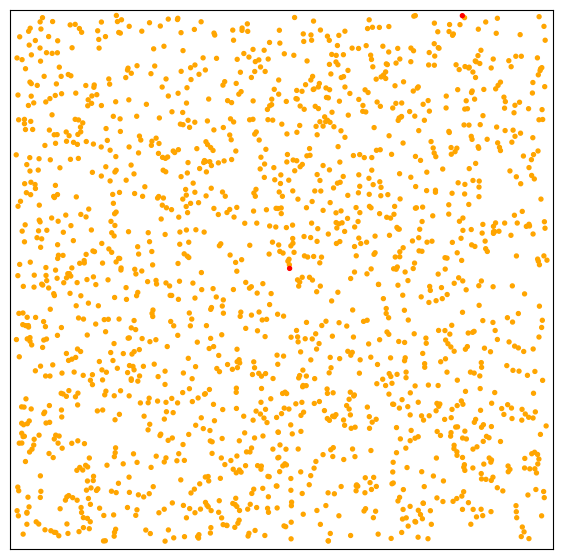
\includegraphics[width=110mm]{1_step.png}
          \caption{初期状態}
          \label{figure:first_step}
        \end{figure}
  \clearpage
  \item 接続可能ノードの探索 \\
        図\ref{figure:second_step}にスタートノードの接続半径を示す.

        ノードの接続条件において,上流ノードはスタートノードに相当する.
        加えて,\ref{2-1}のように,接続範囲内に存在するノードへ情報を送信している状態である.
        
        \indent シミュレーションでは,\ref{2-2},\ref{2-3}の過程をこの時に同時に行っており,上流ノードは接続可能な下流ノードの
        数を保持している.

        \begin{figure}[H]
          \centering
          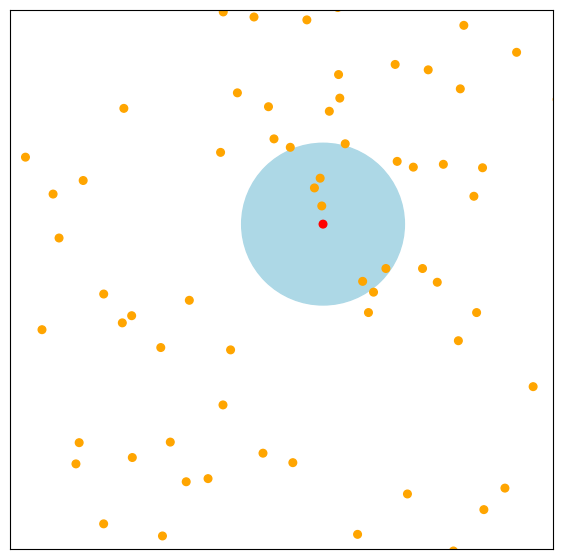
\includegraphics[width=80mm]{2_step.png}
          \caption{接続可能ノードの探索}
          \label{figure:second_step}
        \end{figure}
  \item ノード接続 \\
        図\ref{figure:third_step}に上流ノードが下流ノードとランダムに接続した様子を示す.

        \begin{figure}[H]
          \centering
          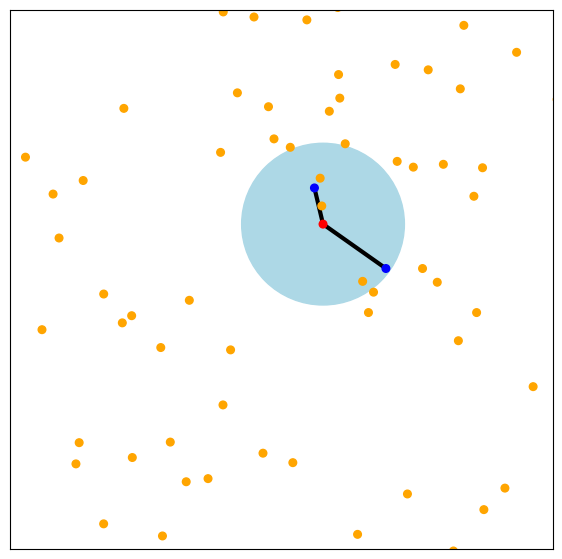
\includegraphics[width=80mm]{3_step.png}
          \caption{ノード接続}
          \label{figure:third_step}
        \end{figure}
  \clearpage
  \item 経路完成 \\
        図\ref{figure:fourth_step}にスタートノードからターゲットノードまでの経路が存在した時の様子を示す.
        経路完成時の通信成功割合の計算式を次に示す.

        \begin{figure}[H]
          \centering
          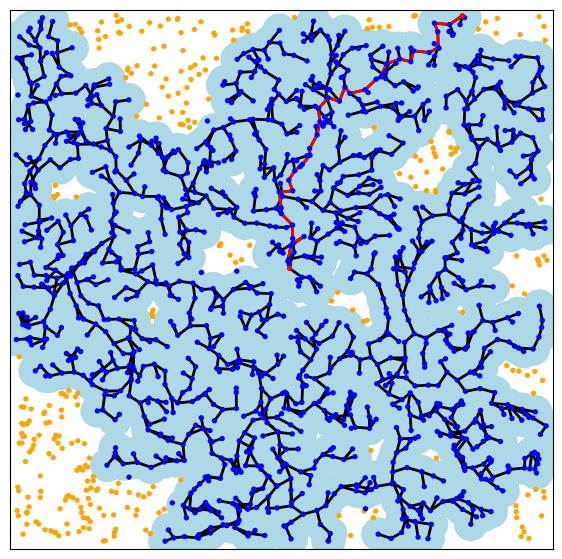
\includegraphics[width=110mm]{4_step.png}
          \caption{経路完成図}
          \label{figure:fourth_step}
        \end{figure}
\end{enumerate}

% ・各都道府県について行う
% ・表にプロットする
% ・先ほどの表より,接続成功割合が著しく低い地域を人口密度が低い地域とし,
% それらでも,安定した通信を行うにはどうすればいいかを書く
% ・あるノードから通信要求が発生したときに枝のように分かれて経路探索が行われる

% ・背景
% 昨年の1月に発生した石川県能登半島地震の時のように,自然災害は何時発生するか不明であり,
% 能登半島地震は実家に帰省する方が必然と多くなるお正月に発生してしままったため,想定よりも
% 多くの方が被災した考えられる.

% ・アドホックネットワークを構築するとき, ノード間の距離が大事になっていると考えている.
% また,距離感はRSSI(Received Signal Strength Indicator) 受信信号強度を用いて距離を推定することは可能だが,
% RSSIを基準に構築を開始すると,設定した閾値に満たすノードがいたとしても,実際には,危険な区域に存在しており,いつ消えてしまうか
% わからない.そこで

%---結果---------------------------------------------------------------------------------------
\clearpage
\section{結果}
本研究内での,人口密度の高低をシミュレーションを通して定義する.
\ref{提案手法}章の提案手法を元に全ての都道府県のに対して閾値$X = 5$の条件で10回シミュレーションを行い,
その平均を図\ref{figure:各都道府県の通信成功割合}のグラフに示す.

\begin{figure}[h]
  \centering
  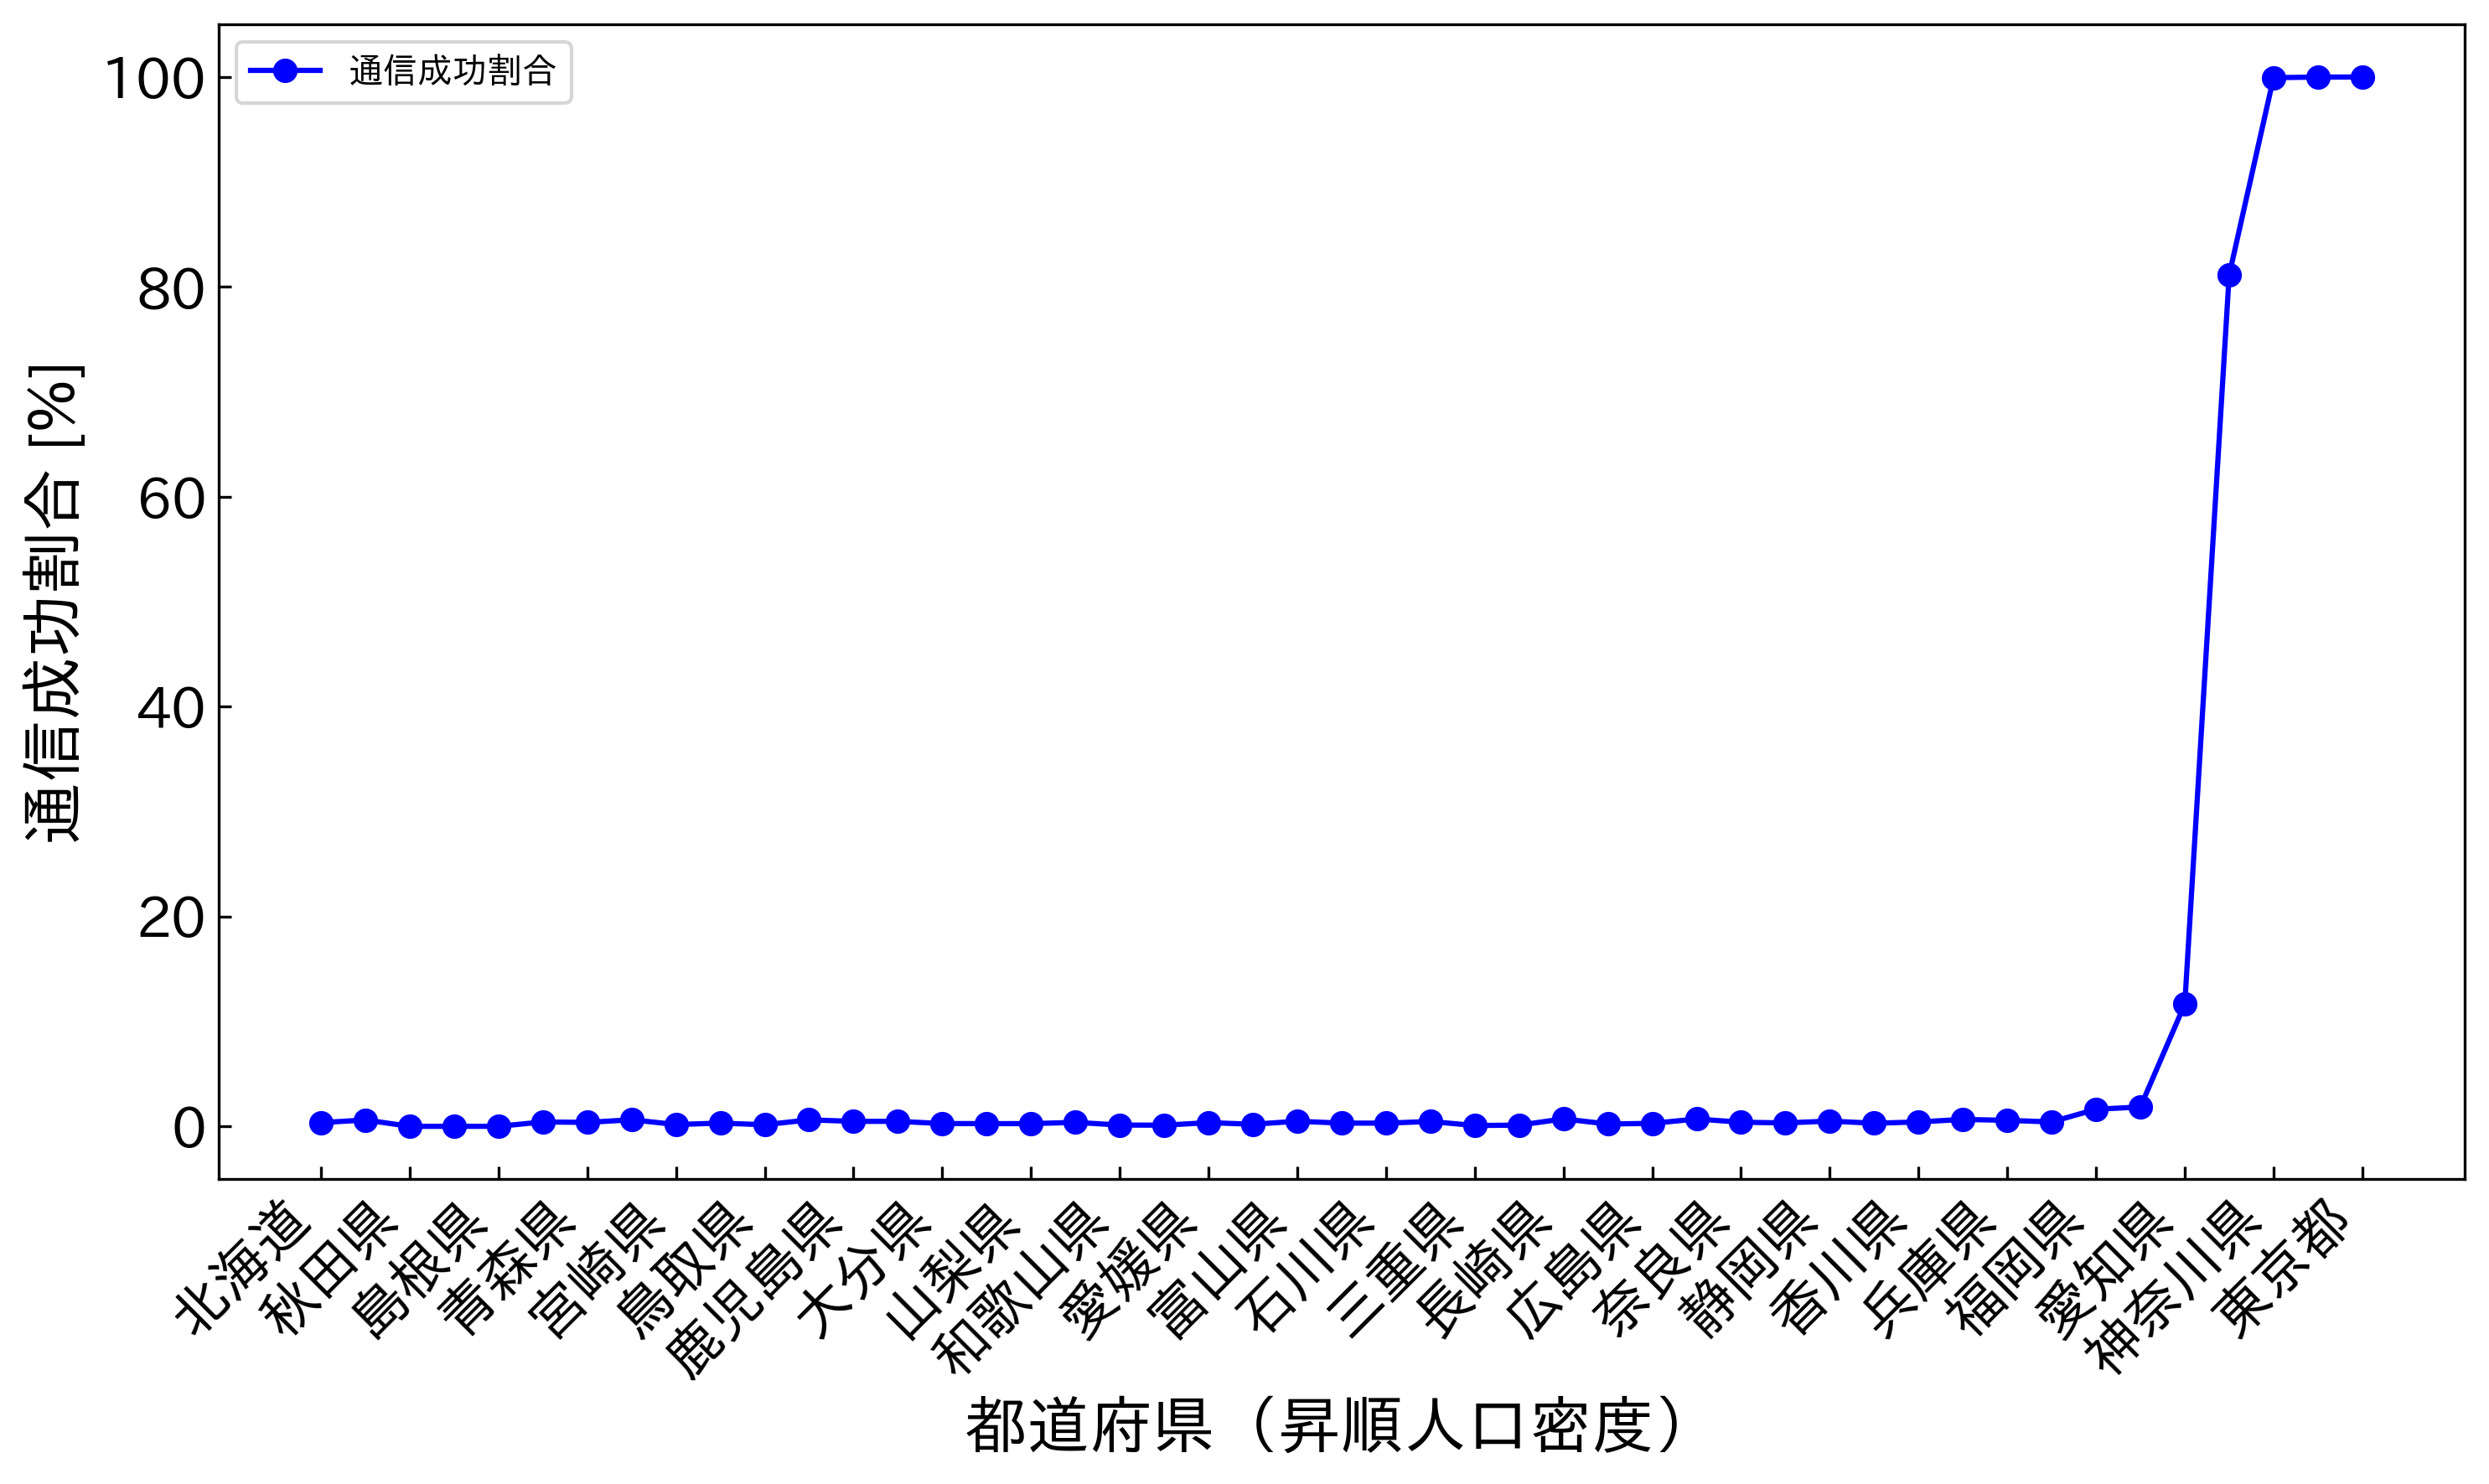
\includegraphics[width=150mm]{通信成功率グラフ.png}
  \caption{各都道府県の通信成功割合}
  \label{figure:各都道府県の通信成功割合}
\end{figure}

\subsection{人口密度が高い地域の場合}
・人口密度が高い地域に対して閾値$X$の値を変化させ,通信成功割合が最も高い$X$を確認する.
・おそらく,人口密度が大きくなると$X$の値が増加する方向にシフトすると思われる.

\subsection{人口密度が低い地域の場合}

%---考察---------------------------------------------------------------------------------------
\clearpage
\section{考察}

%---まとめ---------------------------------------------------------------------------------------
\section{まとめ}

%---参考文献()---------------------------------------------------------------------------------------
\clearpage
% \pagenumbering{gobble}
\addcontentsline{toc}{section}{参考文献}
\bibliography{arxiv}
\bibliographystyle{junsrt}


\end{document}